%====================================================================================================
% ?????
%====================================================================================================
% TCC
%----------------------------------------------------------------------------------------------------
% Autor				: Jasane Schio
% Orientador		: Gedson Faria
% Co-Orientador		: Angelo Darcy
% Instituição 		: UFMS - Universidade Federal do Mato Grosso do Sul
% Departamento		: CPCX - Sistema de Informação
%----------------------------------------------------------------------------------------------------
% Data de criação	: 01 de Outubro de 2015
%====================================================================================================

\chapter{Aplicativo} \label{Cap:Aplicativo}
\section{Tela Principal}
\begin{figure}[!h]
	\centering
	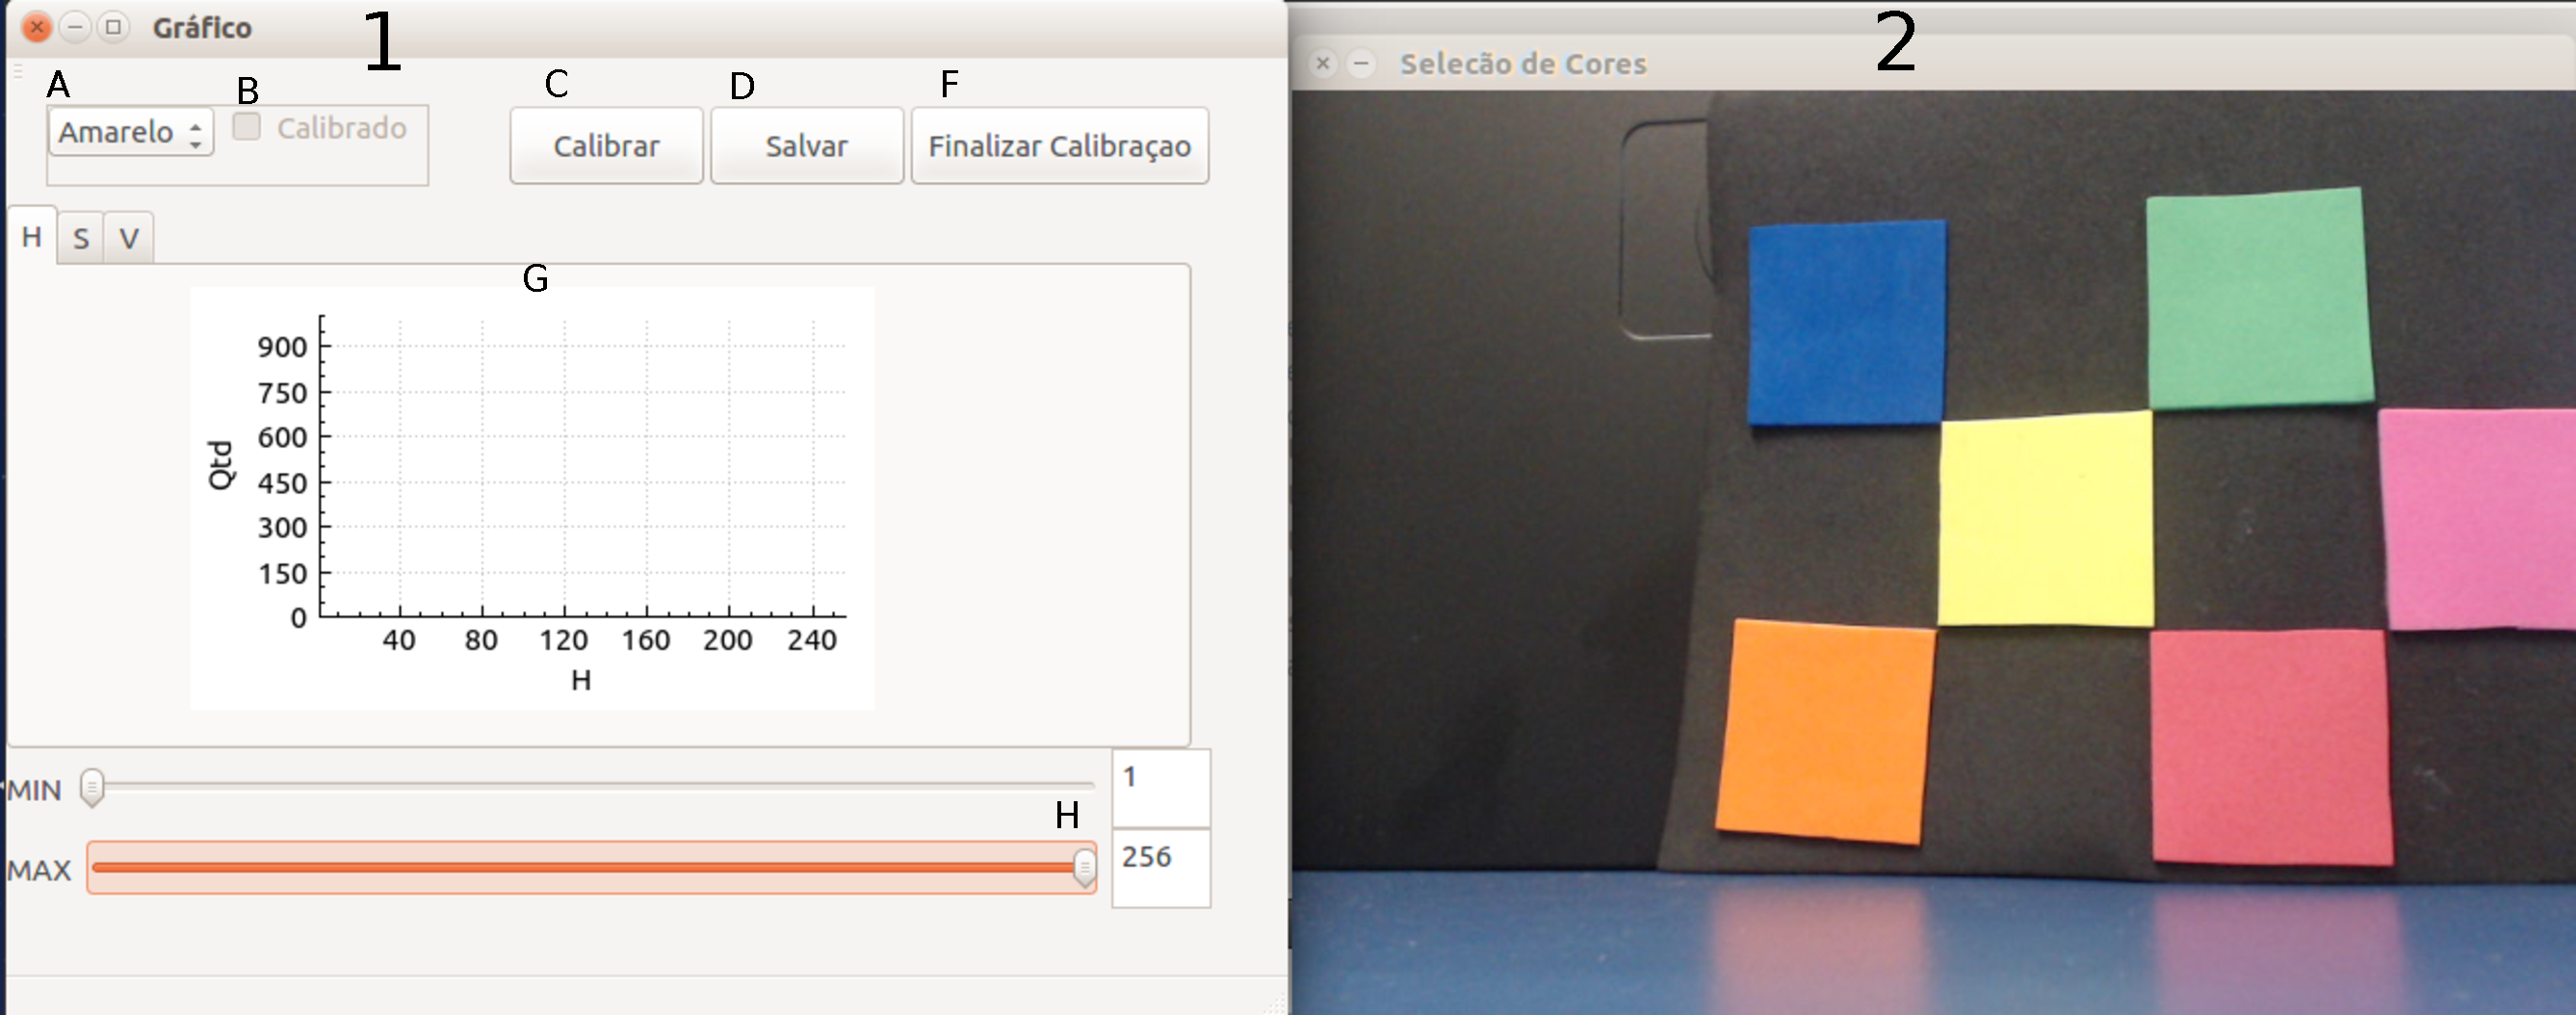
\includegraphics[width=0.98\textwidth]{manual1.pdf}
	(a) Janela 1 \hspace{5cm} (b) Janela 2
	\caption{Janelas do Sistema: Janela 1 e Janela 2 }
	\label{TelanInicial}
\end{figure}
A tela do sistema é formada por duas janelas. Janela 1 é a janela que recebe as interação do usuário, a Janela 2 é composta pela imagem obtida pela câmera, e para ser feita a escolha da cor.
Na Janela 1 possui ações de escolha de cor via Combo Box(A), um Check Box(B) que informa se a cor já foi calibrado ou não. Botões de Calibrar(C), que é usado apos a seleção da cor para a geração do gráfico, Salvar(D), que é usado apos a seleção dos valores para que estes sejam salvos na memoria do aplicativo, e Finalizar Calibração(F) que ira salvar os valores em arquivo. Uma área de gráfico (G) onde são mostrados os valores de ocorrência de H, S e V, cada um em uma aba diferente. A Janela 1 ainda possui um área de seleção dos valores(H), com região MIN e MAX que possui tanto Sliders quando Área de texto para seleção dos valores mínimos e máximos.
 \newpage

\section{Seleção do Objeto Colorido}
\begin{figure}[!h]
	\centering
	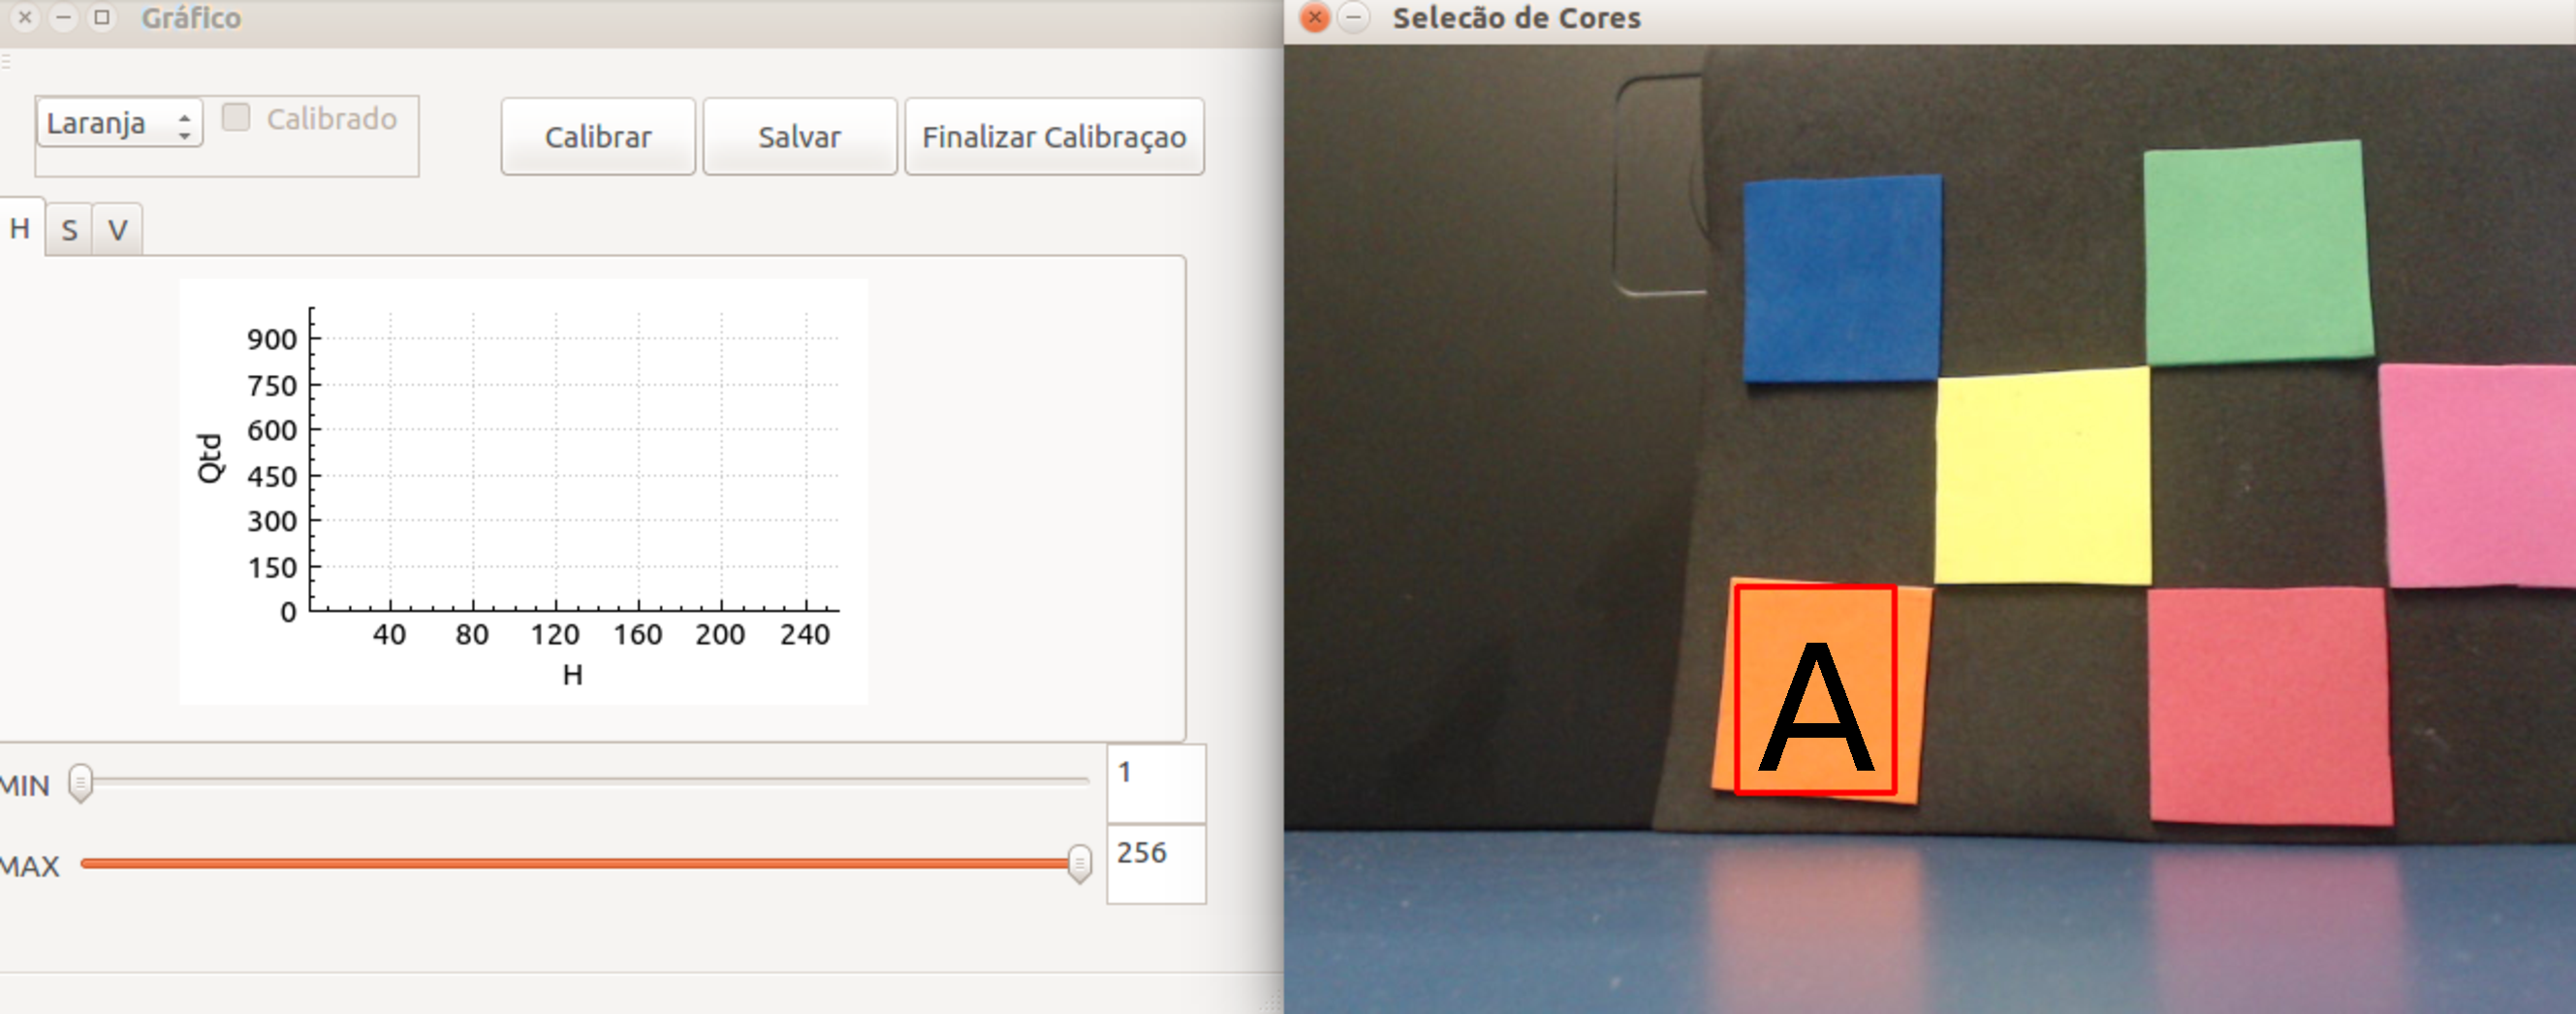
\includegraphics[width=0.98\textwidth]{manual2.pdf}
	\caption{A seleção do ponto com a cor, é obtido pela interação do usuário.}
	\label{SelecaoCor}
\end{figure}
A seleção das cores é feita selecionando, com o ponteiro do mouse clicando na área inicial e arrastando até a área final do objeto correspondente a cor. Um exemplo de seleção de cor ocorre na Figura 4.2 em A onde é selecionada a cor Laranja. Apos seleção da cor é necessário apertar no botão Calibrar para assim ser feito os cálculos dos valores HSV dos pixels e ser gerado o gráfico.

\section{Geração de Gráfico}
\begin{figure}[!h]
	\centering
	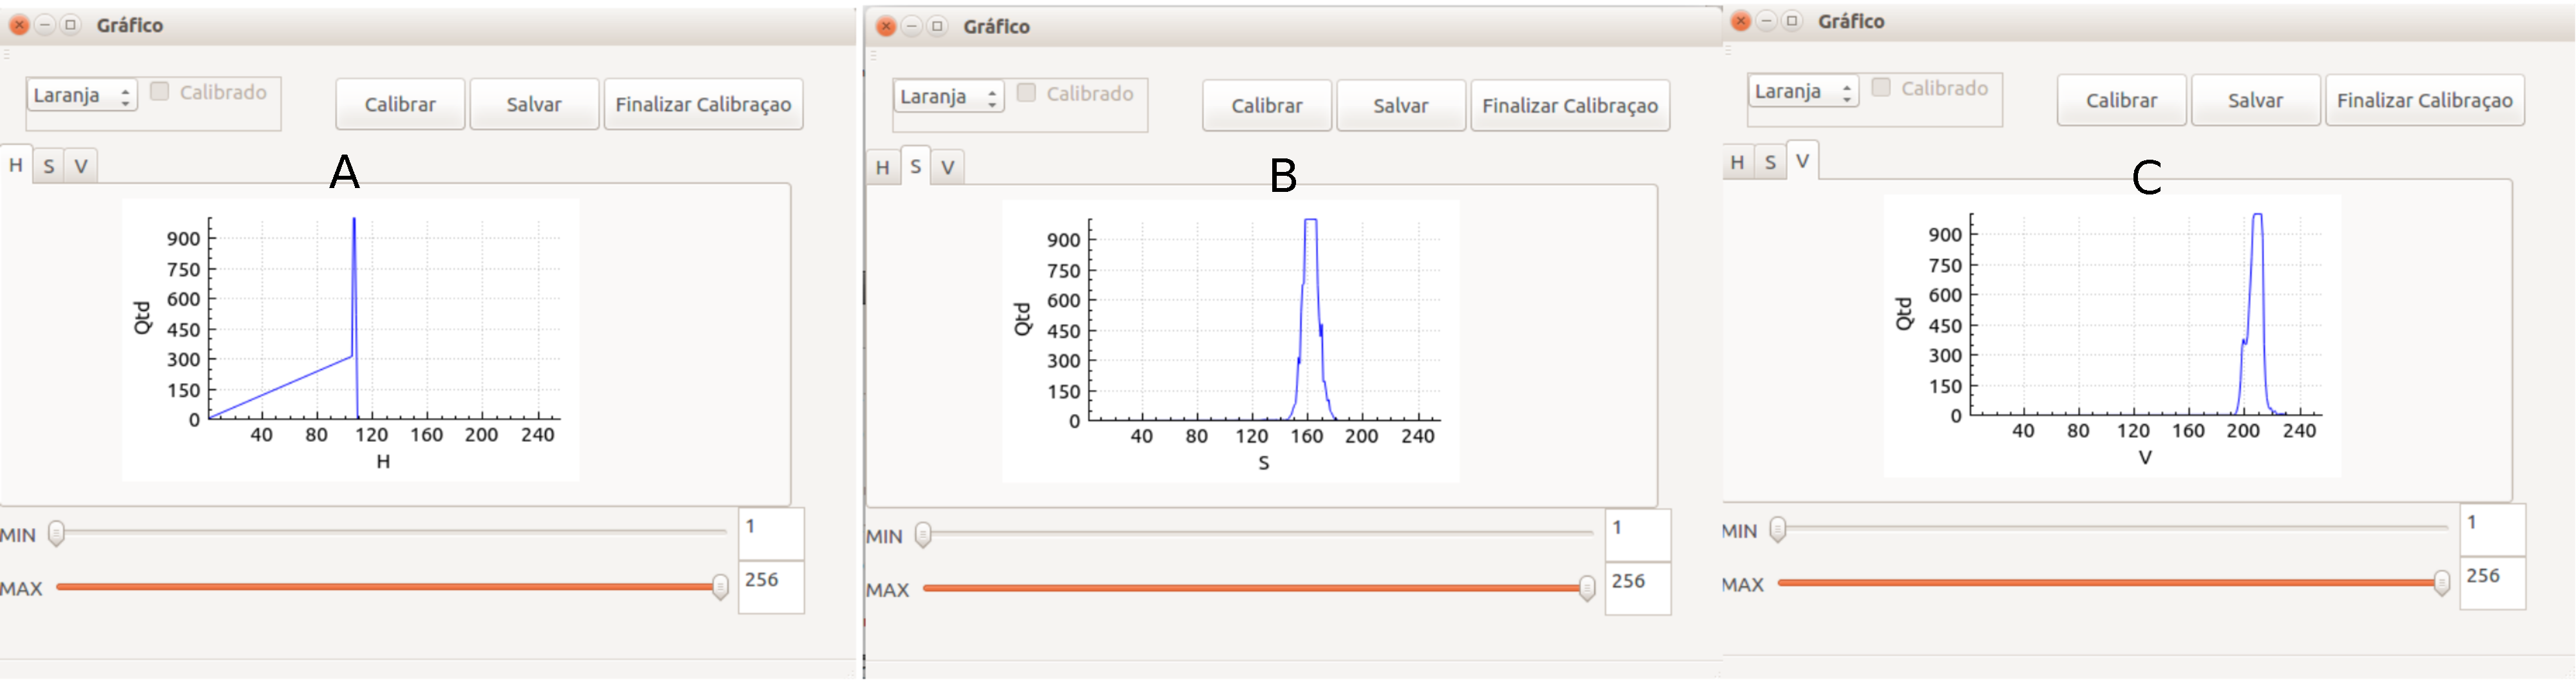
\includegraphics[width=0.98\textwidth]{manual3.pdf}
	\caption{Gráfico gerado após seleção dos pontos de cor.}
	\label{GraficoGerado}
\end{figure} 
Quando se aperta o botão Calibrar são gerados os 3 Gráficos de ocorrência de valor de H(A), S(B) e V(C), um em cada aba. No gráfico são vistos quais os valores que possuem mais ocorrência, para assim ser feita a seleção.
\newpage
\section{Seleção de Minimos e Maximos}
\begin{figure}[!h]
	\centering
	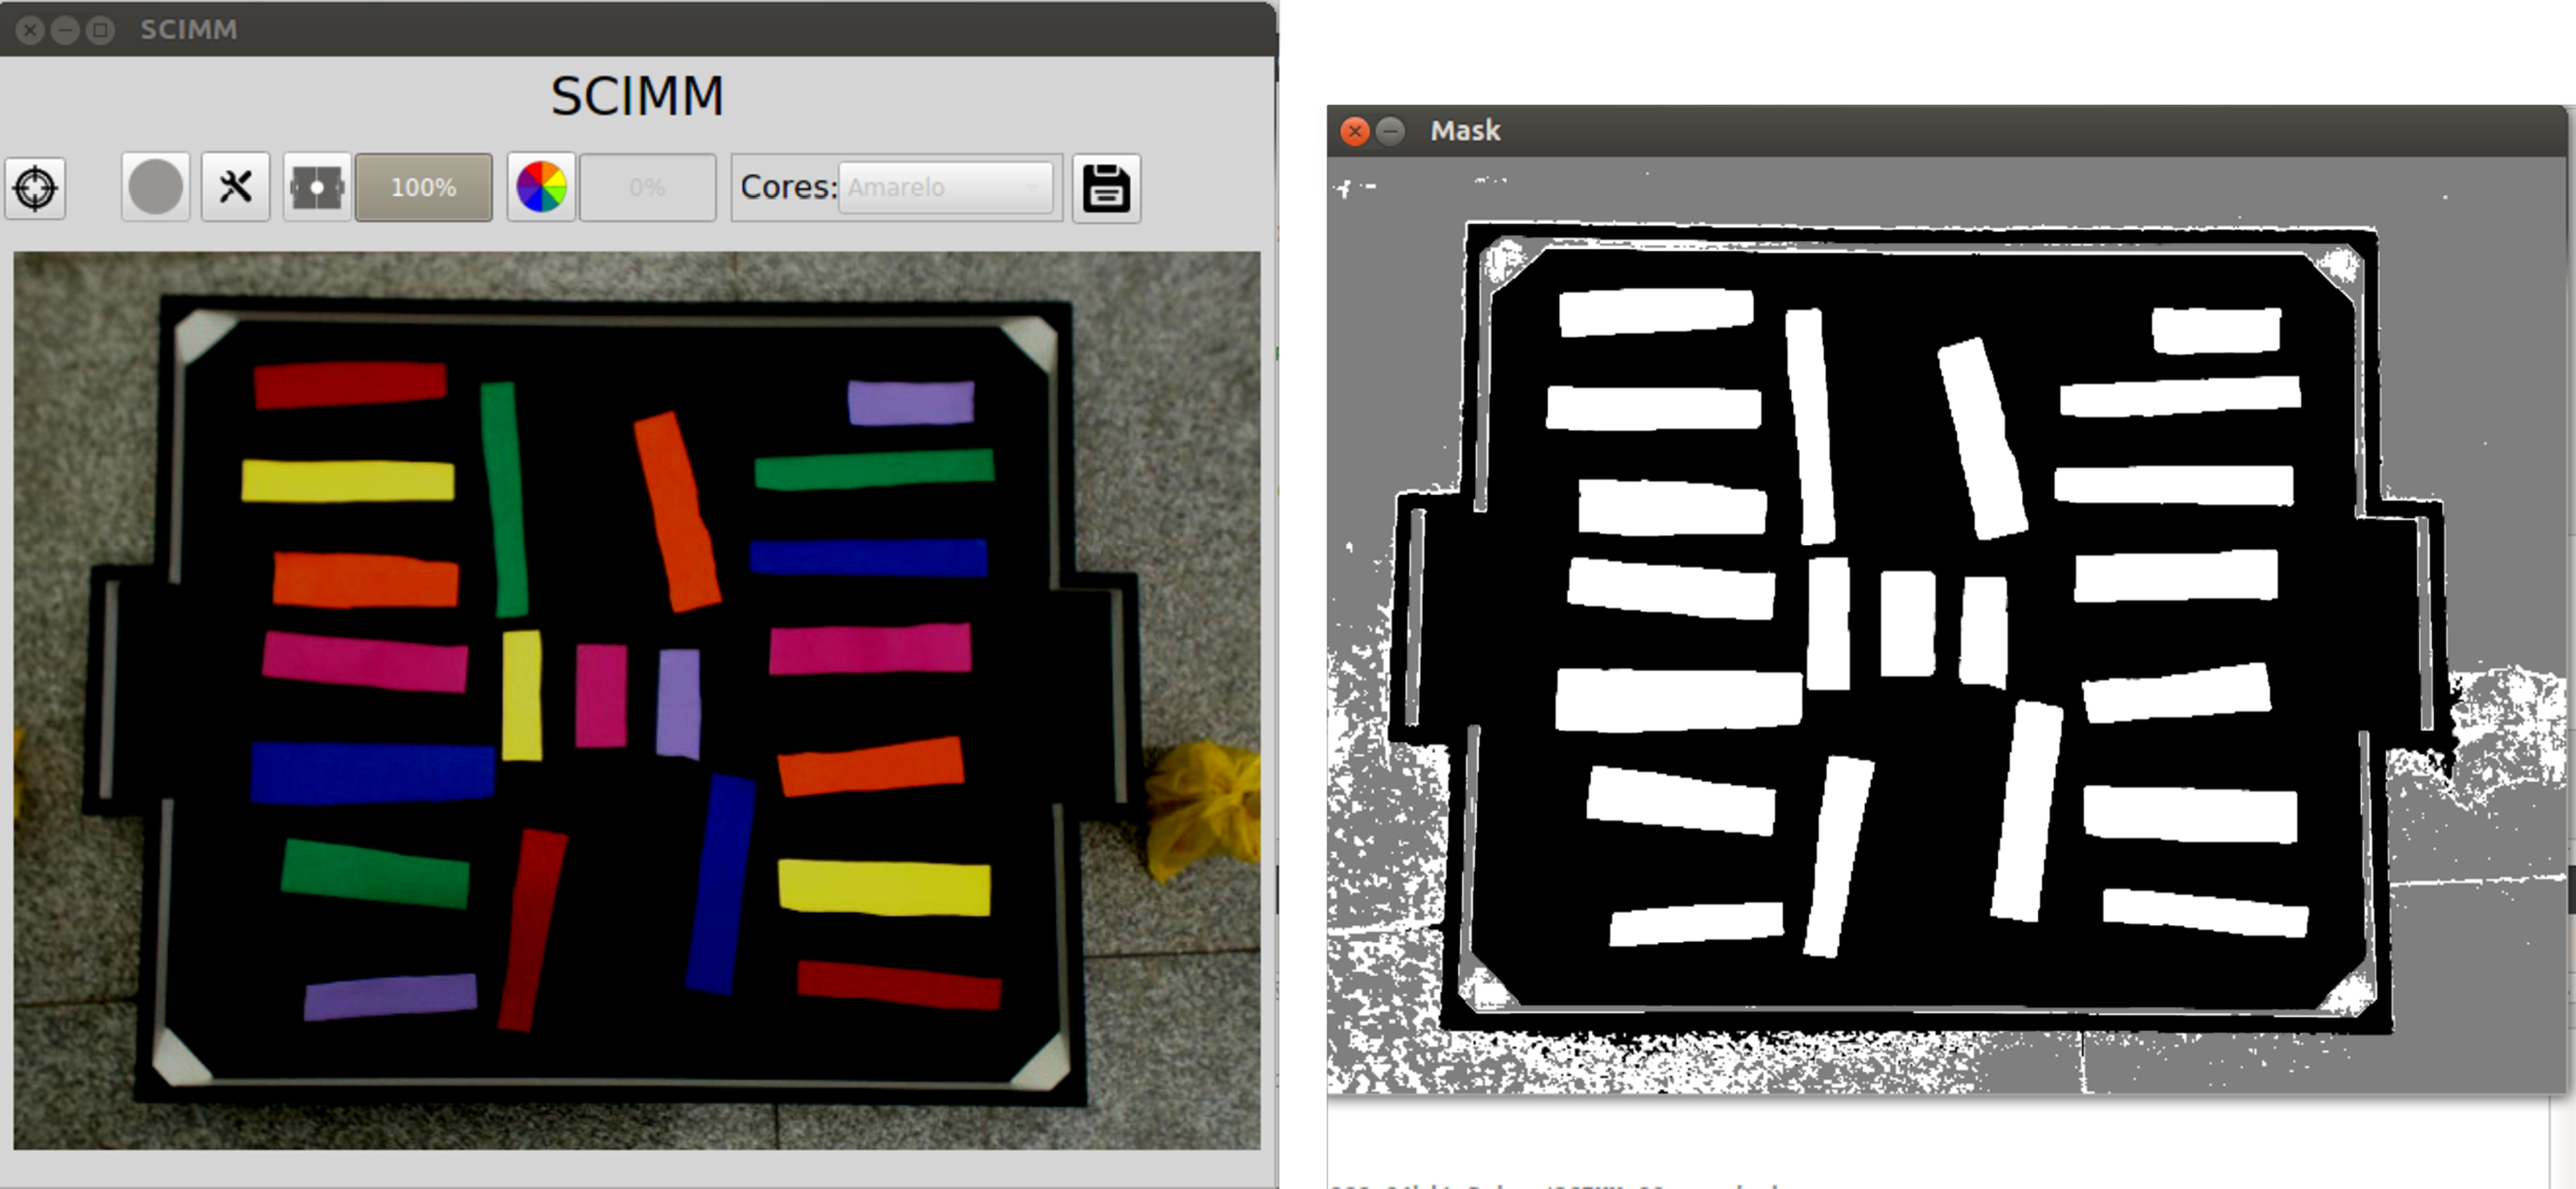
\includegraphics[width=0.98\textwidth]{passo3.pdf}
	\caption{Gráfico após escolhas de mínimos e máximos.}
	\label{GraficoGerado2}
\end{figure}
Usando os Sliders ou Entrada de Texto(explicados na sessão 4.1) são selecionados os valores mínimos e máximos para H, S e V. Durante a seleção dos valores o gráfico é atualizado para melhor visualização das ocorrências.
\section{Arquivo Final}

Arquivo gerado apos valores serem selecionados e salvos. Para cada cor selecionado são feitas duas linhas, a primeira contendo os valores mínimos e a segunda os valores máximos, no inicio de cada linha há o índice da cor.
  \begin{figure}[!h]
  	\centering
  	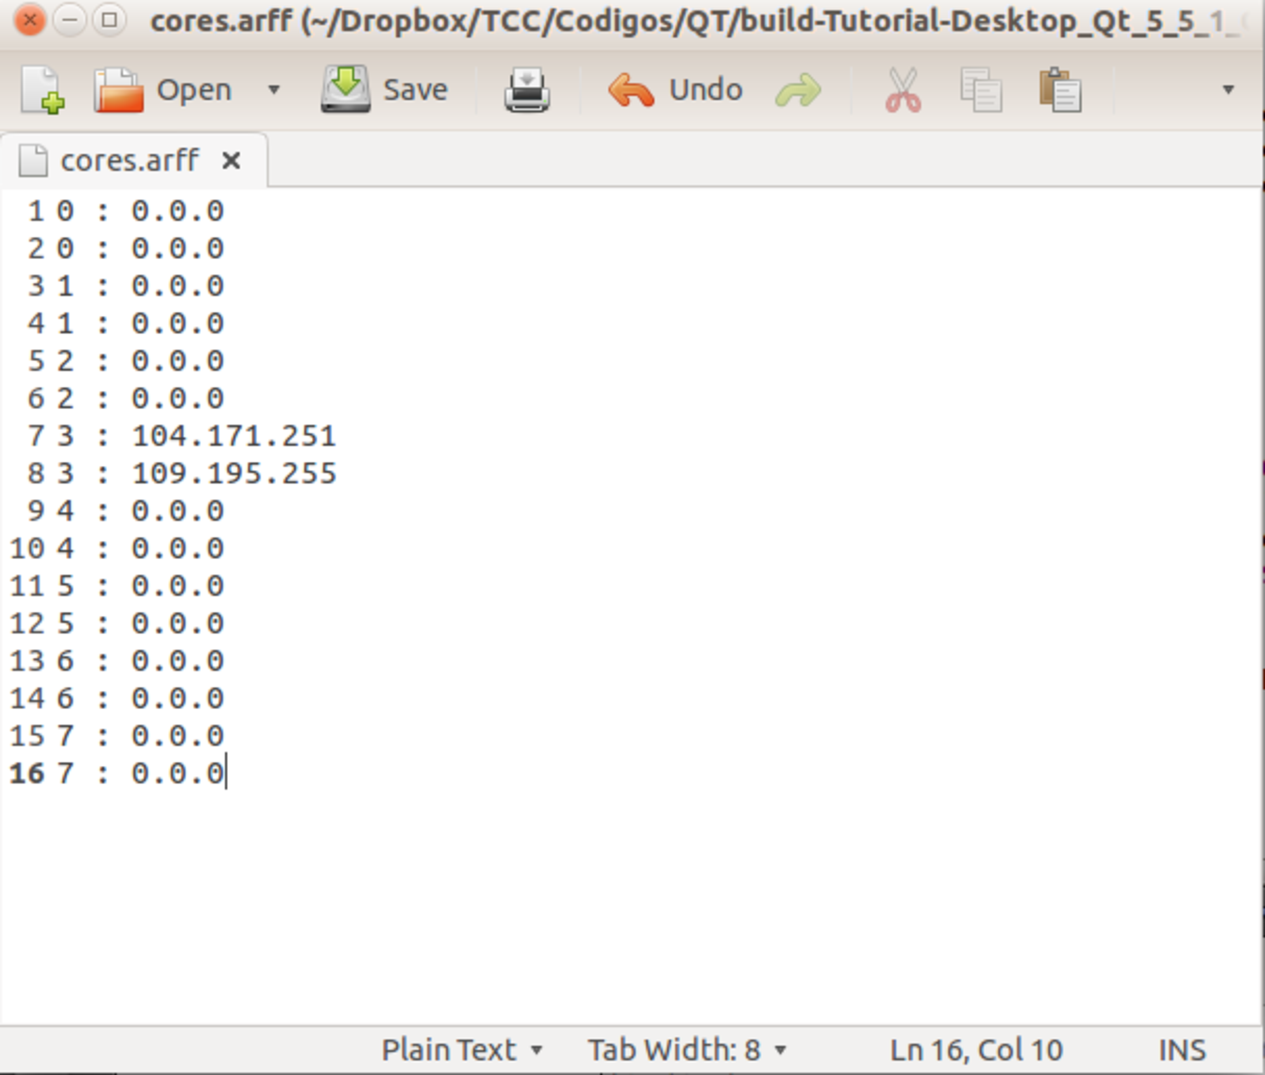
\includegraphics[width=0.7\textwidth]{arquivoResultado.pdf}
  	\caption{Arquivo com minimo e máximo dos valores HSV para cada cor.}
  	\label{ArquivoValores}
  \end{figure}
  \newpage
	
\newpage
